\section{Implementation of the FVM in 1D}
The code to solve the SWE in 1D using FVM is based on the Godunov scheme with the exact Riemann solver.
The exact solution of the Riemann problem is found by using the Riemann invariants and the Rankine-Hugoniot conditions~\cite{trento_course}.


\section{True solution}
In this section, we present how the so-called true solution is found in the code by solving the Riemann problem exactly.
The true solution is found by solving the Riemann problem exact, with 5000 cells, and distinguishing between the wetbed or drybed case, and also identifying the shock and rarefaction waves.
First we caculate the wave speeds for the left and right states, respectively, as
\begin{align*}
    c_L = \sqrt{g h_L}, \quad c_R = \sqrt{g h_R},
\end{align*}
which are used to determine the critical water height $h_{\text{crit}}$ as
\begin{align*}
    h_{\text{crit}} = (u_R - u_L) - 2(c_L + c_R).
\end{align*}
If either $h_L \leq 0$ or $h_R \leq 0$, we are in a drybed case.
If $h_{\text{crit}} \geq 0$ it means the water depth is somehow critical, and we are in a drybed case,
If none of the above conditions are met, we are in a wetbed case.
Summarized:
\begin{align*}
    \begin{cases}
        \text{Dry-bed case} & \text{if }  h_L \leq 0, \quad  h_R \leq 0 \text{ or } h_{\text{crit}} \geq 0, \\
        \text{Wet-bed case} & \text{otherwise}.
    \end{cases}
\end{align*}
For a dry bed case, we then identify where the dry is located, i.e., if the left side is dry, the right side is dry, or the middle is dry, and calculate the wave speeds accordingly.
For a wet bed case, we compute the characteristics $h_*$ and $u_*$ for the star region.
We then identify the shock and rarefaction waves, and calculate the wave speeds for the left and right states, respectively.

FLOW-DIAGRAM.

\section{FVM in 2D}

\subsection{the MUSCL scheme}
The MUSCL (Monotone Upwind Scheme for Conservation Laws), second order accurate in space and time.
High-order total variation diminishing (TVD) scheme.
We use the finite volume update:
\begin{align}
    \mathbf{U}_{i,j}^{n+1} = \mathbf{U}_{i,j}^n - \frac{\Delta t}{\Delta x}(\mathbf{F}_{i+1,j} - \mathbf{F}_{i,j}) - \frac{\Delta t}{\Delta y}(\mathbf{G}_{i,j-1} - \mathbf{G}_{i,j}).
\end{align}






\section{Data generation}
We use the Matlab script: SWE1D-data-generation to generate the data for the training and testing of the neural network, and the Python script: data-generation to load and visualize the data.
The data generation is done by solving the SWE in 1D using the FVM with the Godunov scheme and the exact Riemann solver.
We use Gaussian functions with parametric extension~\cite{Gaussian} to generate the initial conditions, that is, functions on the form
\begin{align*}
    h(x,0) &= a \exp{\left(\frac{-{(x-\mu)}^2}{2\sigma^2}\right)}, \\
\end{align*}
where $a$ is the amplitude of the Gaussian, $\mu$ is the mean value, and $\sigma$ is the standard deviation.
We solve the 1D SWE with the following parameters:
\begin{itemize}
    \item $N = 200$ cells,
    \item From $t = 0.0$ to $t_{\text{end}} = 1.0$,
    \item $x \in [0, 1]$,
    \item $u(x,0) = 0$,
    \item $b(x) = 0.0$,
    \item $g = 9.81$ and
    \item $\sigma = 0.1$.
\end{itemize}
The value of $\mu$ is varied to generate different initial conditions, as seen in Figure~\ref{fig:data_generation_initial}.
\begin{figure}[H]
    \centering
    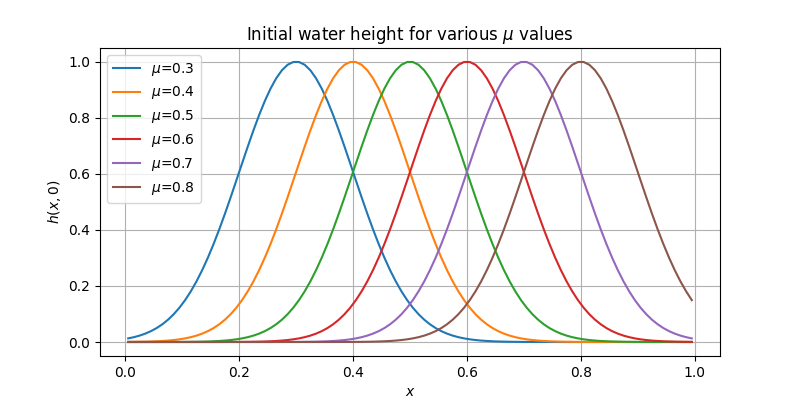
\includegraphics[width=0.8\textwidth]{C:/Users/Matteo/Shallow-Water-Equations/plots/data_generation_initial.png}
    \caption{Initial conditions for the data generation.}\label{fig:data_generation_initial}
\end{figure}


\section{Data Copernicus}

\begin{figure}[H]
    \centering
    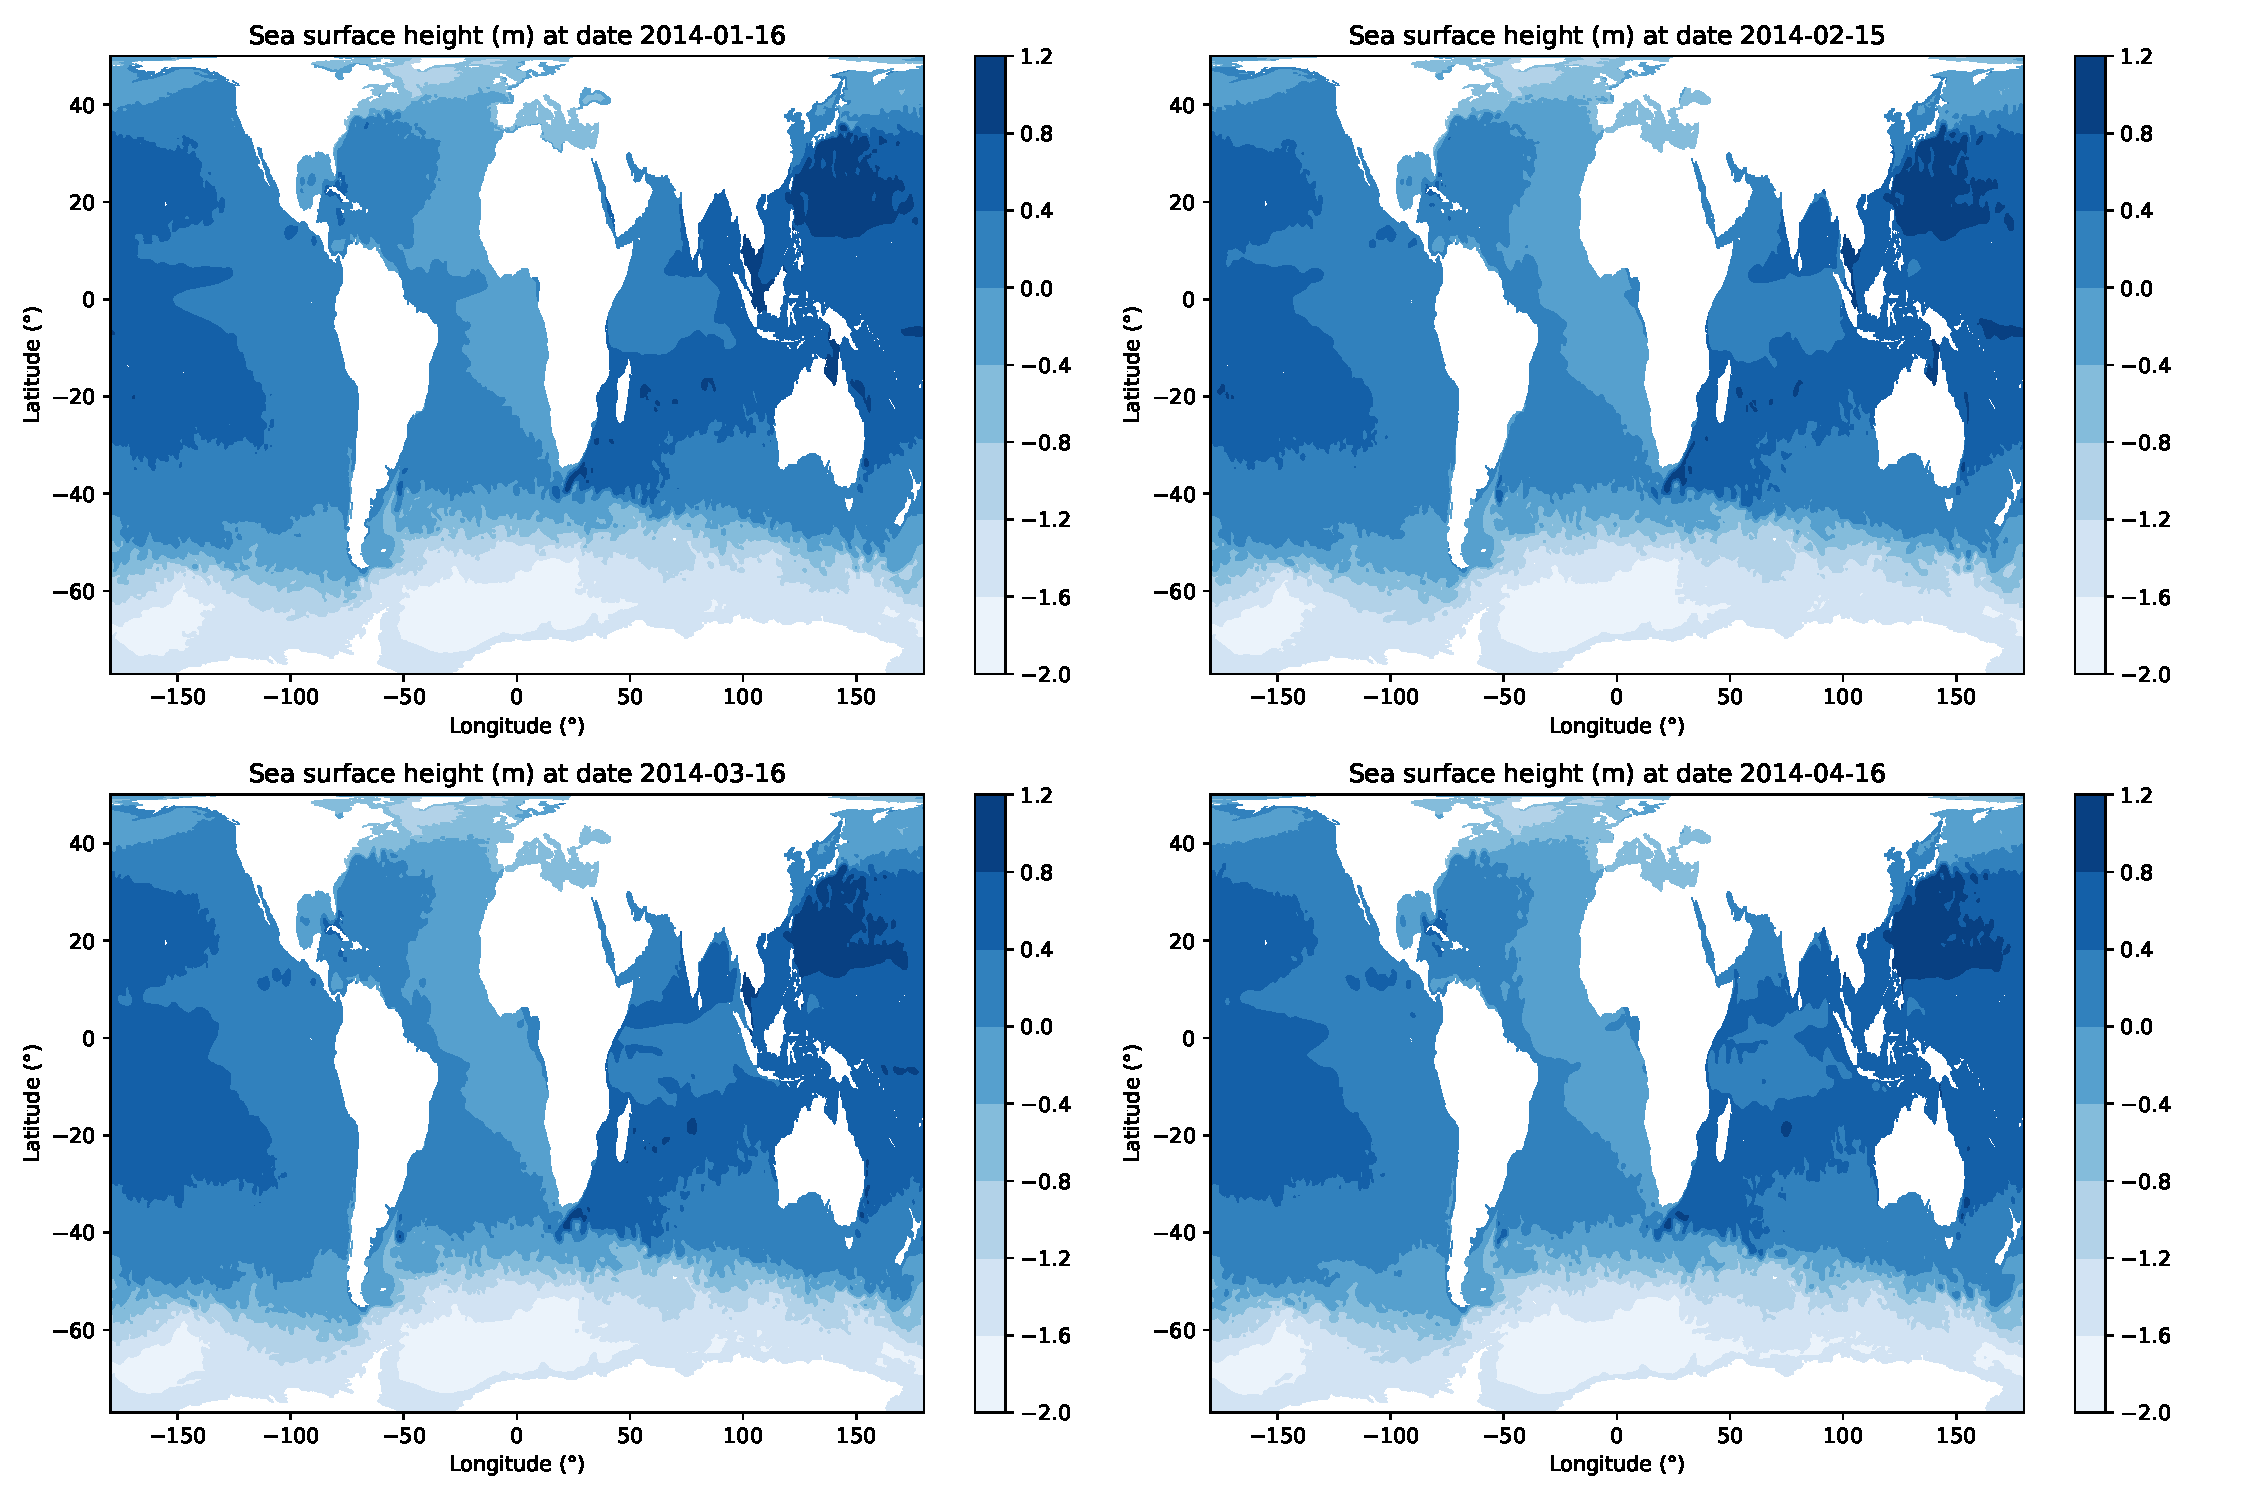
\includegraphics[width=0.95\textwidth]{C:/Users/Matteo/Shallow-Water-Equations/plots/ssh_field.pdf}
    \caption{Sea surfae height as the diffference from reference sea surface height for the months jan-apr 2014.}\label{fig:copernices-ssh}
\end{figure}


